\apendice{Especificación de diseño}

\section{Introducción}

En este apartado desglosaremos las estrategias de diseño tomadas en consideración: \textit{conjuntos de datos, clases, procedimientos..}, para el cumplimiento de los requerimientos funcionales y no funcionales reseñados en el primer apartado.

\section{Diseño de datos}

\subsection{Entidades}

\begin{itemize}
    \item \textbf{Usuario (\textit{User})}: Consta de un identificador auto-incrementado como clave primaria, así como atributos para el \textit{nombre}, su \textit{correo electrónico}, contraseña \textit{encriptada} y fechas de \textit{creación} y \textit{modificación}.
    \item \textbf{Planificación:} Consta de un identificador como clave primaria, el identificador del usuario que la creó (\textit{FK}) y la fecha de creación.
    \item \textbf{Predicción:} Sigue la misma estructura de atributos que la entidad \textit{Planificación}.
\end{itemize}

\newpage
\subsection{Diagrama Relacional}

\imagen{diagRel}{Diagrama Relacional}


\subsection{Diagrama E-R}

\imagen{diagERD}{Diagrama Relacional}

\newpage

\section{Diseño procedimental}

En este apartado, se desgranan los procedimientos que permiten especificar el funcionamiento interno de las aplicaciones.

Existen muchos tipos de diagramas que pueden representar estas funcionalidades, aunque para esta ocasión hemos elegido los \textit{diagramas de interacción} y, dentro de éstos, los de \textit{secuencia}  \cite{Britton2005IdentifyingDiagrams}. En él, registraremos el comportamiento de nuestro sistema mediante una secuencia de eventos \textbf{ordenados por tiempo}.

En primer lugar, reflejaremos la acción de \textit{modificar el perfil} de un usuario en nuestro interfaz, con la secuencia de acciones representadas en el diagrama \ref{fig:UsuarioEst}

\imagen{UsuarioEst}{Diag Int-Seq: Modificar Perfil de Usuario}

Mostramos ahora las acciones que puede realizar el usuario \textbf{administrador} sobre las acciones de creación, modificación y eliminación de usuario, como vemos en \ref{fig:AdminUs}

\imagen{AdminUs}{Diag Int-Seq: Gestión de Usuarios}

Dentro de este proyecto, podemos diferenciar dos \textbf{funcionalidades:} Planificación de Intervenciones y Predicción de duración, tanto de forma \textit{independiente} como \textit{interrelacionada} (llamada de una funcionalidad a otra en caso de ser requerida).

El usuario puede \textit{crear, visualizar o eliminar} una determinada \textbf{predicción}, siguiendo el siguiente esquema (partiendo del supuesto de un inicio de sesión exitoso), en el diagrama \ref{fig:PredUs}

\imagen{PredUs}{Diag Int-Seq: Gestión de Predicciones}

De modo similar, gestionaremos las \textbf{planificaciones}, con las acciones previstas en el diagrama \ref{fig:PlanUs}


\imagen{PlanUs}{Diag Int-Seq: Gestión de Planificaciones}


\section{Diseño arquitectónico}

Al haber optado para el despliegue por el desarrollo tanto de una API como proveedora de servicios como por una \textit{aplicación web} que sirva de GUI para los usuarios clientes, se han seguido los patrones \textbf{cliente-servidor} y \textbf{MVC} (\textit{Modelo Vista Controlador}) en el diseño de la arquitectura de este proyecto software.

\subsection{Modelo Cliente-Servidor}

La arquitectura cliente-servidor, nos presenta una serie de \textit{ventajas de diseño}\cite{Rana2022HighDesign}:

\begin{enumerate}[label=\Alph*]
    \item Facilita el \textbf{mantenimiento}, dado que los roles se encuentran distribuidos a lo largo de varios servidores independientes.
    \item Permite una fácil \textbf{escalabilidad} y modularidad del sistema.
    \item Los datos están centralizados, de forma que varios clientes distintos pueden acceder desde diversas localizaciones. La existencia de recursos compartidos facilita a su vez la gestión, modificación y \textbf{reutilización} de módulos software.
\end{enumerate}

Siguiendo este modelo, y aplicado al sistema particular desarrollado en el proyecto, podríamos definir \textbf{dos modelos} cliente-servidor:

\begin{itemize}
    \item La comunicación entre el \textbf{interfaz web y la API} proveedora de servicios de predicción y planificación, referenciada en la figura \ref{fig:diagCSAPI}
\imagen{diagCSAPI}{Esquema Cliente-Servidor de APP-WEB y API}
    \item Por otra parte, definiremos la comunicación entre los \textbf{usuarios clientes} y la \textbf{aplicación web distribuida}, como vemos en la imagen \ref{fig:diagCSAPP}
\imagen{diagCSAPP}{Esquema Cliente-Servidor de Usuario y APP-WEB}
\end{itemize}

\subsection{Modelo-Vista-Controlador}

En este caso, debido a la implementación de una base de datos, así como de dos servicios computacionales \textit{externalizados}, parece ser adecuado separar la \textbf{vista} del \textbf{modelo de datos} subyacente \cite{Pop2014DesigningDevelopment}.

Aquí, tanto el interfaz de usuario, como la lógica de negocio y la integración con otros sistemas y subsistemas han sido desarrolladas en Python, y desplegadas en servidores externos a partir de las funcionalidades que ofrece Amazon Web Services:

\begin{itemize}
    \item \textbf{AWS Elastic Container Services}: para ejecutar los servidores y las tareas.
    \item \textbf{AWS RDS}: para almacenamiento y lógica de base de datos relacional.
    \item \textbf{AWS Elastic Container Registry:} para almacenamiento persistente de los \textit{contenedores} construidos a partir de los ficheros fuente de la aplicación.
\end{itemize}

\imagen{MVC}{Modelo-Vista-Controlador}

Podemos comprobar cómo el \textit{Framework Flask} es el encargado de aportar la solución al desarrollo del interfaz web siguiendo este modelo, comportándose como el controlador y aislando el modelo de datos de la vista.

\subsection{Diseño de Paquetes}

Para facilitar la \textit{legibilidad} del código, tratamos de ofrecer una estructuración del sistema en dos \textit{subsistemas} (API y APP-WEB), comunicados según el patrón cliente-servidor, de forma distribuida, y dividiendo los paquetes de cada uno de ellos siguiendo un \textit{enfoque por características}.

En este enfoque, todas las clases requeridas para una misma funcionalidad se encuentran en el mismo paquete, consiguiendo una \textbf{alta cohesión} entre las clases de un mismo paquete y un \textbf{acoplamiento reducido} entre diferentes paquetes.

Así, podemos comprobar la notación de los paquetes y cómo se distribuyen según su funcionalidad de forma jerárquica y caracterizable, diferenciando el diagrama de paquetes para el subsistema API \ref{fig:packages_API} y el del interfaz web \ref{fig:packages_APPWEB}
\begin{landscape}
\begin{figure}
    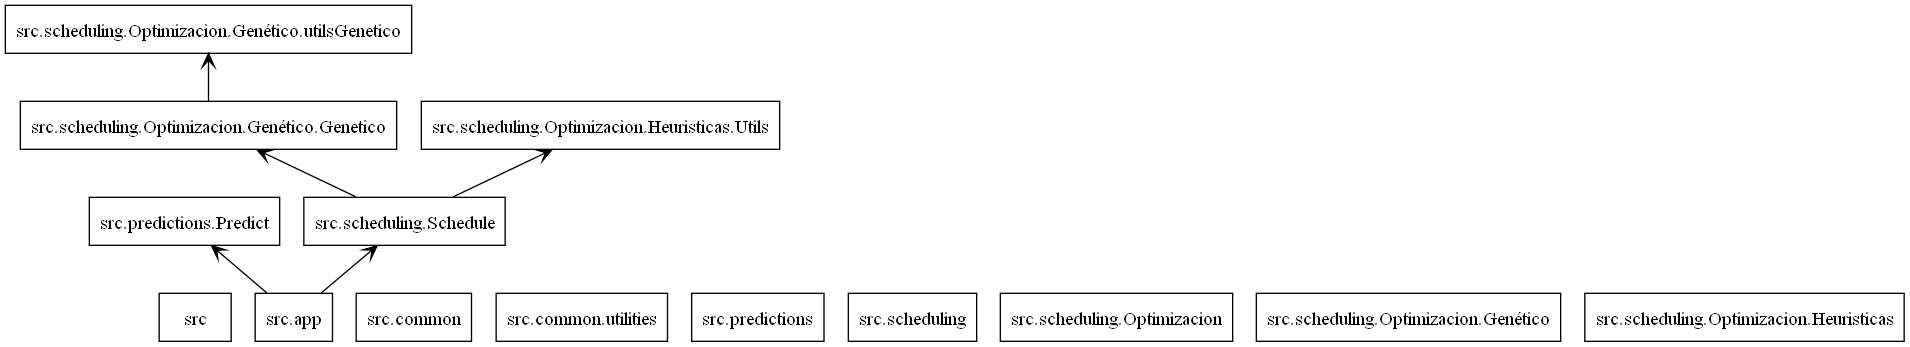
\includegraphics[scale = 0.7, width = 20cm]{packages_API}
    \caption{Diagrama de paquetes API}
    \label{fig:packages_API}
\end{figure}
\end{landscape}

\begin{landscape}
\begin{figure}
    \centering
    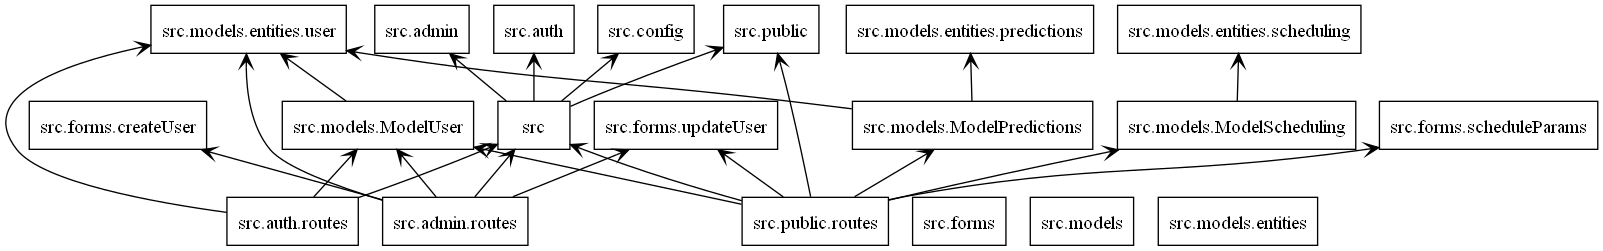
\includegraphics[scale = 0.4]{packages_APPWEB}
    \caption{Diagrama de paquetes APP Web}
    \label{fig:packages_APPWEB}
\end{figure}
\end{landscape}

Por último, podemos ver el diagrama de clases desglosadas dentro de cada subsistema, y localizar su posición en el paquete a partir de los diagramas de paquetes mostrados con anterioridad, siguiendo la notación \textit{\textbf{dot}}, tanto para la API (\ref{fig:classes_API_1}, \ref{fig:classes_API_2}) como para la aplicación web (\ref{fig:classes_APPWEB_1}, \ref{fig:classes_APPWEB_2})

\begin{landscape}
\begin{figure}
    \centering
    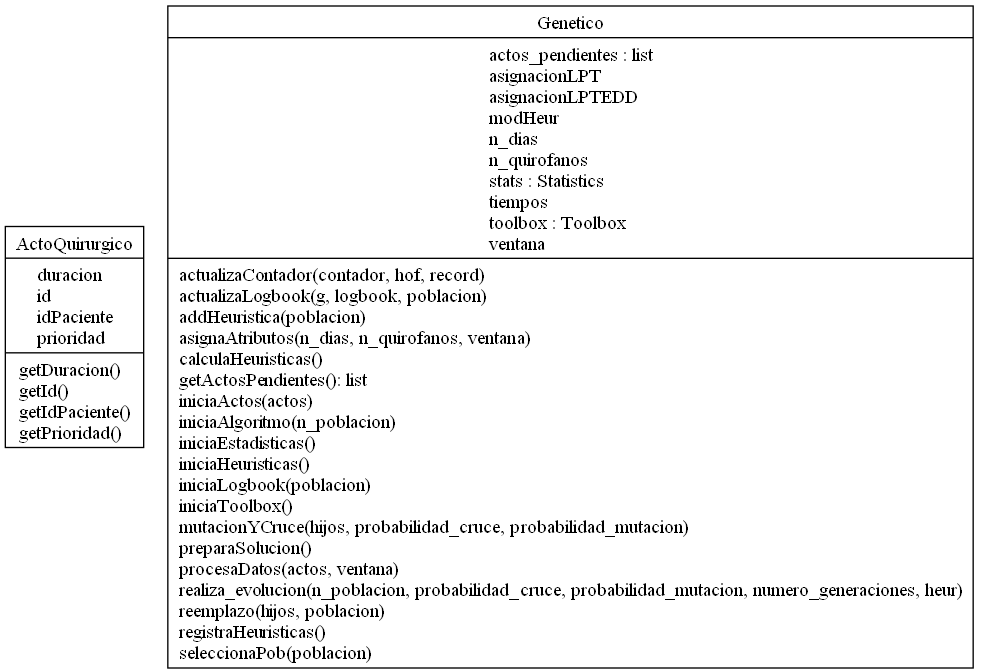
\includegraphics[scale = 0.6]{classes_API_1}
    \caption{Diagrama de clases del subsistema API - 1}
    \label{fig:classes_API_1}
\end{figure}
\begin{figure}
    \centering
    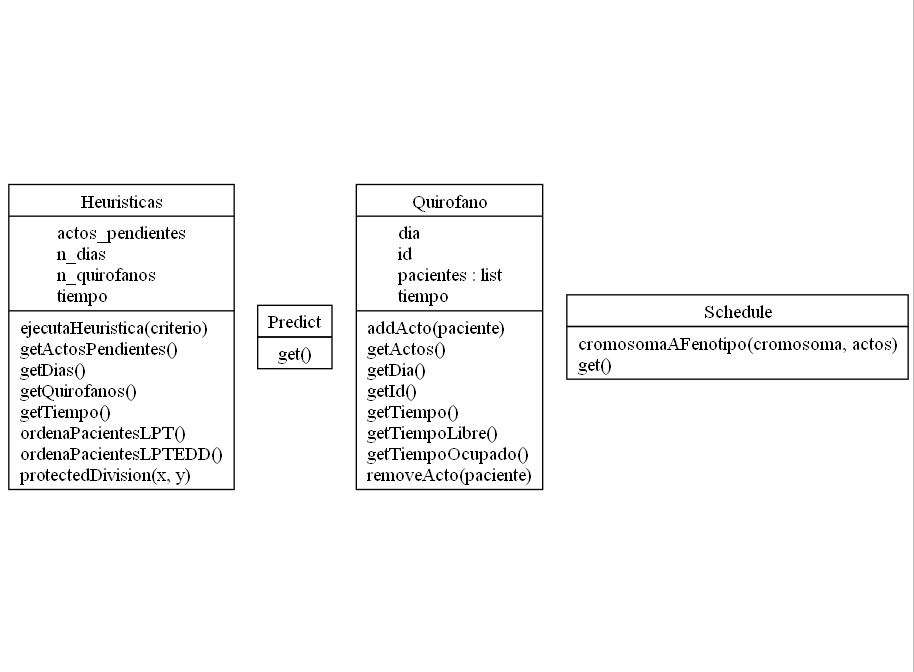
\includegraphics[scale = 0.6]{classes_API_2}
    \caption{Diagrama de clases del subsistema API - 2}
    \label{fig:classes_API_2}
\end{figure}
\end{landscape}

\begin{landscape}
\begin{figure}
    \centering
    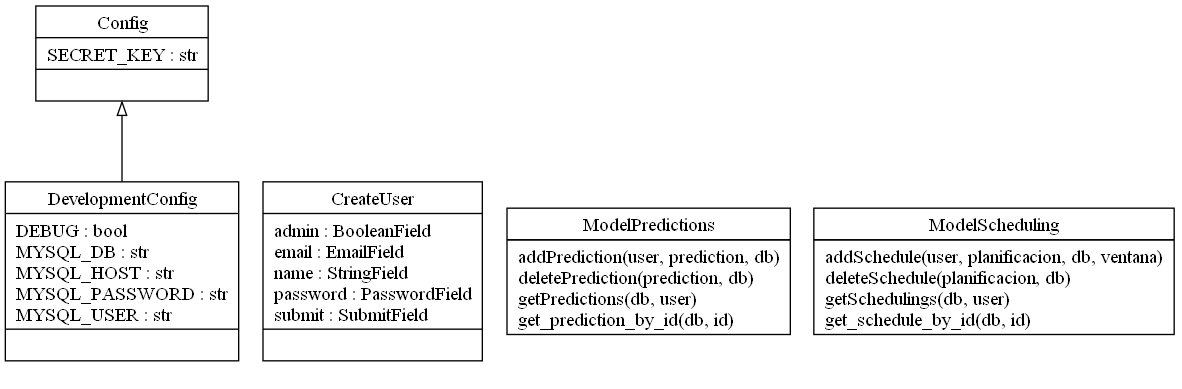
\includegraphics[scale = 0.6]{classes_APPWEB_1}
    \caption{Diagrama de clases del subsistema APP-WEB - 1}
    \label{fig:classes_APPWEB_1}
\end{figure}
\begin{figure}
    \centering
    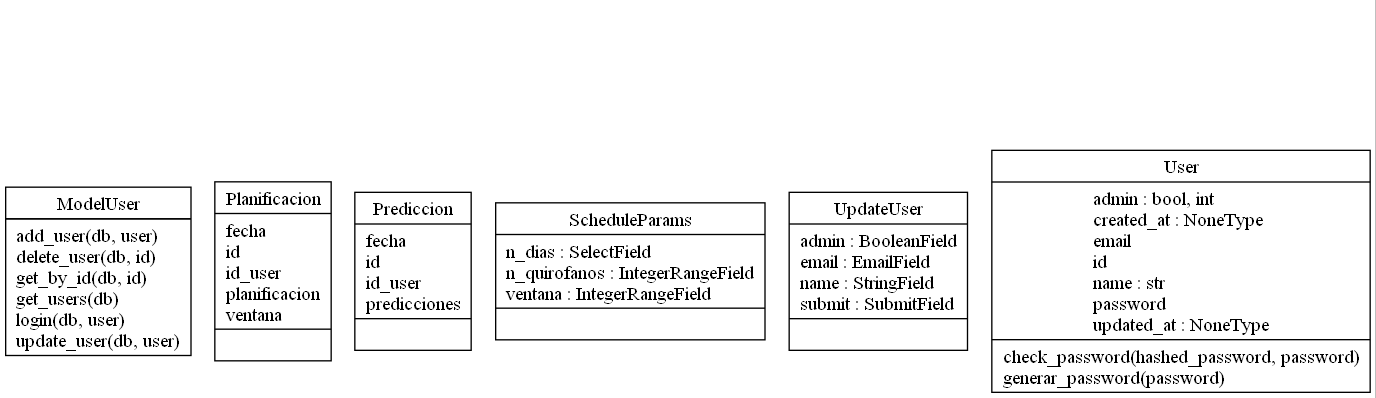
\includegraphics[scale = 0.5]{classes_APPWEB_2}
    \caption{Diagrama de clases del subsistema APP-WEB - 2}
    \label{fig:classes_APPWEB_2}
\end{figure}
\end{landscape}

\subsection{Diseño de despliegue}

Se muestra a continuación, de forma esquemática, el diagrama de \textbf{despliegue UML} de nuestro proyecto, en la figura \ref{fig:Despliegue}

\imagen{Despliegue}{Diagrama de despliegue UML}